\documentclass[12pt]{article}
\setlength{\oddsidemargin}{0in}
\setlength{\evensidemargin}{0in}
\setlength{\textwidth}{6.5in}
\setlength{\parindent}{0in}
\setlength{\parskip}{\baselineskip}
\usepackage{amsmath,amsfonts,amssymb}
\usepackage{graphicx}
\usepackage{enumitem}
\usepackage[]{algorithmicx}
\usepackage{amsthm}
\usepackage{fancyhdr}
\pagestyle{fancy}
\setlength{\headsep}{36pt}
\usepackage{tkz-berge}
\usetikzlibrary{positioning, automata}

\usepackage{hyperref}

\theoremstyle{remark}
\newtheorem*{solution}{Solution}

\newcommand{\makenonemptybox}[2]{%
%\par\nobreak\vspace{\ht\strutbox}\noindent
\item[]
\fbox{% added -2\fboxrule to specified width to avoid overfull hboxes
% and removed the -2\fboxsep from height specification (image not updated)
% because in MWE 2cm is should be height of contents excluding sep and frame
\parbox[c][#1][t]{\dimexpr\linewidth-2\fboxsep-2\fboxrule}{
  \hrule width \hsize height 0pt
  #2
 }%
}%
\par\vspace{\ht\strutbox}
}
\makeatother

\begin{document}

\lhead{{\bf CSCI 3104, Algorithms \\ Problem Set 8a (14 points)} }
\rhead{Name: Luna McBride \\ ID: 107607144 \\ {\bf Profs.\ Hoenigman \& Agrawal\\ Fall 2019, CU-Boulder}}
\renewcommand{\headrulewidth}{0.5pt}

\phantom{Test}

\begin{small}
\textit{Advice 1}:\ For every problem in this class, you must justify your answer:\ show how you arrived at it and why it is correct. If there are assumptions you need to make along the way, state those clearly.
\vspace{-3mm} 

\textit{Advice 2}:\ Verbal reasoning is typically insufficient for full credit. Instead, write a logical argument, in the style of a mathematical proof.\\
\vspace{-3mm} 

\textbf{Instructions for submitting your solution}:
\vspace{-5mm} 

\begin{itemize}
	\item The solutions \textbf{should be typed} and we cannot accept hand-written solutions. \href{http://ece.uprm.edu/~caceros/latex/introduction.pdf}{Here's a short intro to Latex.}
	\item You should submit your work through \href{https://www.gradescope.com/courses/59294}{\textbf{Gradescope}} only.
	\item If you don't have an account on it, sign up for one using your CU email. You should have gotten an email to sign up. If your name based CU email doesn't work, try the identikey@colorado.edu version. 
	\item Gradescope will only accept \textbf{.pdf} files (except for code files that should be submitted separately on Gradescope if a problem set has them) and \textbf{try to fit your work in the box provided}. 
	\item You cannot submit a pdf which has less pages than what we provided you as Gradescope won't allow it. 
\end{itemize}
\vspace{-4mm} 
\end{small}

\hrulefill
\pagebreak


\begin{enumerate}
\item (2 pts) If the arrays, $A=[12, 14, 23, 34]$ and $B=[11, 13, 22, 35]$ are merged, list the indices in $A$ and $B$ that are compared to each other. For example, $A[0], B[0]$ means that $A[0]$ is compared to $B[0]$.
\begin{solution}
$\newline$ A[0]B[0], A[0]B[1], A[1]B[1], A[1]B[2], A[2]B[2], A[2]B[3], A[3]B[3]. $\newline$ Added to array in later while loop: B[3] $\newline$ End: Arr=[11, 12, 13, 14, 22, 23, 34, 35] 
\end{solution}

\item (3 pts) Illustrate how to apply the QuickSelect algorithm to find the $k = 4$th smallest element in the given array: \texttt{A = [5, 3, 4, 9, 2, 8, 1, 7, 6]} by showing the recursion call tree.
\begin{solution}
$\newline$ $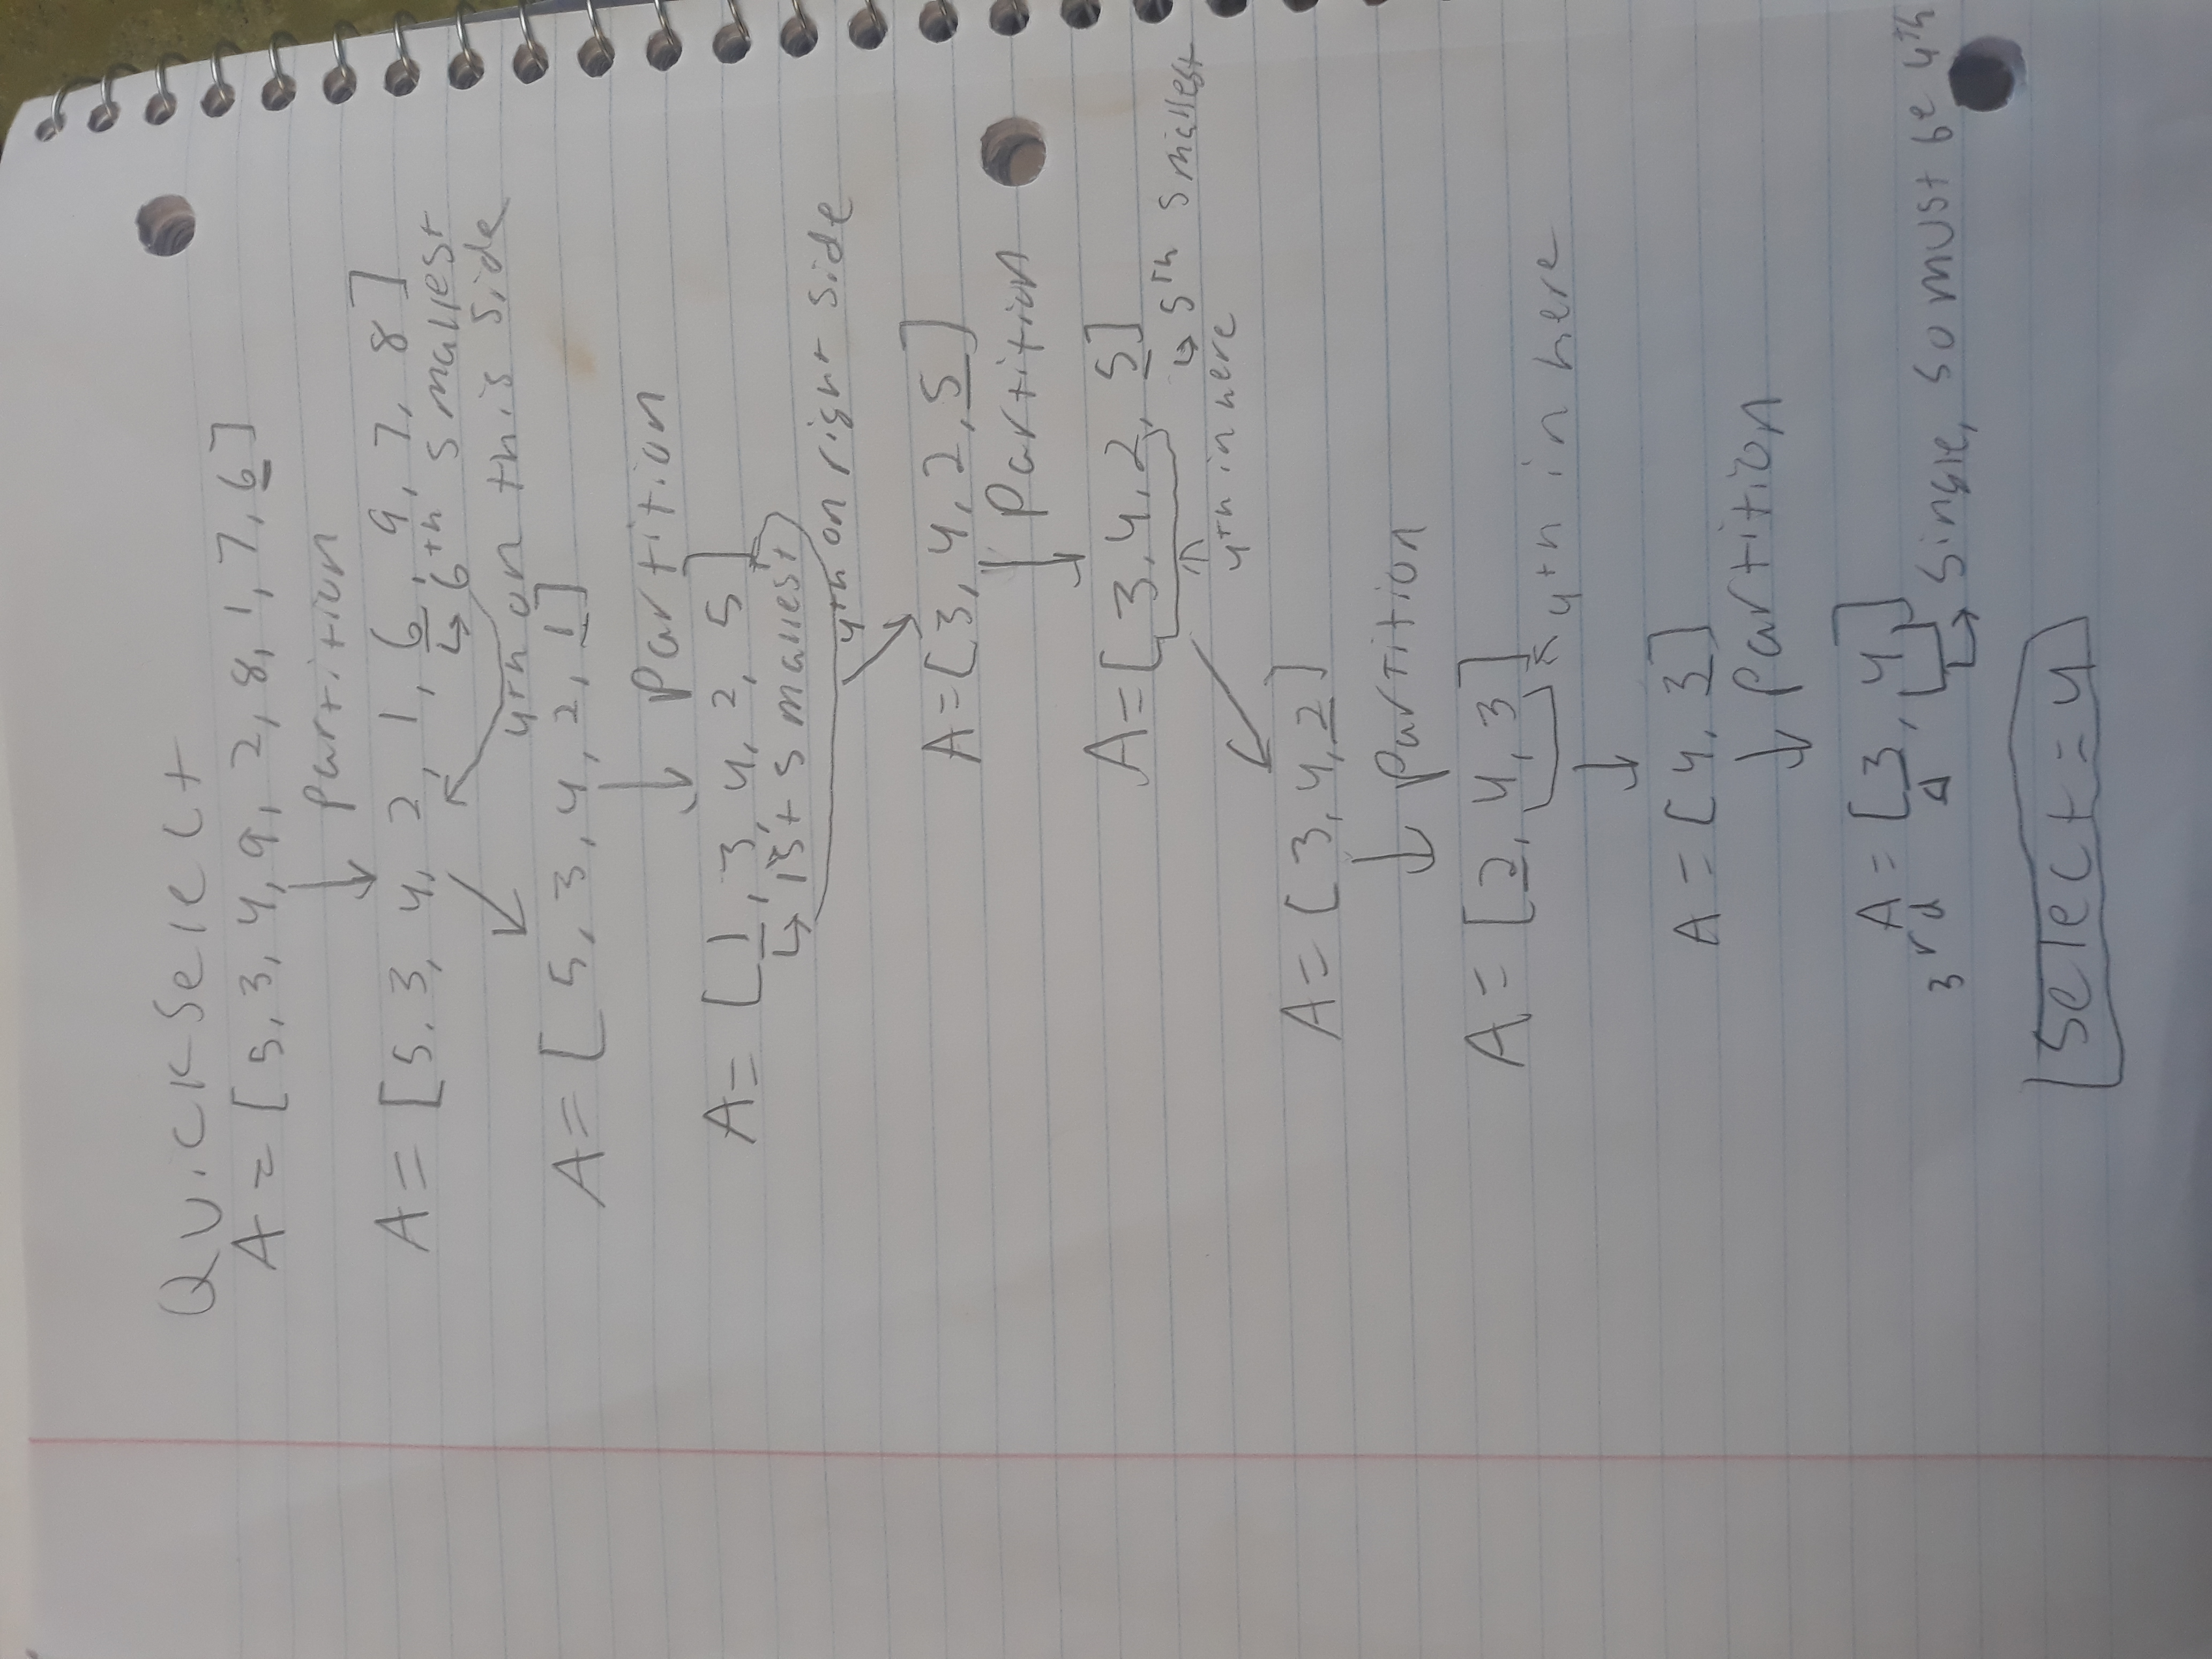
\includegraphics[width=\textwidth,angle=-90]{Select}$
\end{solution}
\pagebreak
\item (1 pt) Explain in 2-3 sentences the purpose of the Median of Medians algorithm.
\begin{solution}
$\newline$ Median of Medians is used to guarentee the average case of a quicksort. It splits the array into arrays of 5, obtains the medians of those, and then gets the median of the medians (hence the name). This is then used as a pivot, as it gets as close to the center as it can and, thus tries for the best case run of the sort.
\end{solution}

\item (4 pts) Illustrate how to apply the Median of Medians algorithm (A Deterministic QuickSelect algorithm) to find the $4$th largest element in the following array: \texttt{A = [6, 10, 80, 18, 20, 82, 33, 35, 0, 31, 99, 22, 56, 3, 32, 73, 85, 29, 60, 68, 99, 23, 57, 72, 25]}.
\begin{solution}
$\newline$ B=[6, 10, 80, 18, 20], C=[82, 33, 35, 0, 31], D=[ 99, 22, 56, 3, 32], $\newline$ E=[ 73, 85, 29, 60, 68], F=[99, 23, 57, 72, 25] $\newline \newline$ B=[6, 10, 18, 20, 80], C=[0, 31, 33, 35, 82], D=[3, 22, 32, 56, 99], $\newline$ E=[29, 60, 68, 73, 85], F=[23, 25, 57, 72, 99] $\newline \newline$ Medians: 18, 33, 32, 68, 57. $->$ 18, 32, 33, 57, 68. $\newline$ Median: 33 $\newline \newline$ Sort with pivot 33: A = [6, 10, 18, 20, 25, 0, 31, 22, 3, 32, 29, 23, |33|, 82, 80, 73, 85, 99, 60, 68, 99, 35, 57, 72, 56] (Largest, so right side next) $\newline \newline$ A=[82, 80, 73, 85, 99, 60, 68, 99, 35, 57, 72, 56] $\newline \newline$ B=[82, 80, 73, 85, 99], C=[ 60, 68, 99, 35, 57], D=[72, 56]$\newline \newline$ B=[73, 80, 82, 85, 99], C=[35, 57, 60, 68, 99] D=[56, 72]$\newline \newline$ Medians= 82, 60, 56 (in case of 2, I choose lower) $\newline$ Median=60 $\newline \newline$ Sort with Pivot 60: A=[56, 35, 57, |60|, 99, 82, 68, 99, 80, 73, 72, 85] $\newline \newline \newline \newline \newline$ A=[ 99, 82, 68, 99, 80, 73, 72, 85] $\newline \newline$ B=[99, 82, 68, 99, 80], C=[73, 72, 85] $\newline \newline$ B=[68, 80, 82, 99, 99], C=[72, 73, 85] $\newline \newline$ Medians: 82, 73 $\newline$ Median=73 $\newline \newline$ A=[68, 72, |73|, 99, 80, 85, 82, 99] $\newline \newline$ A=[99, 80, 85, 82, 99] $\newline$ A=[80, 82, 85, 99, 99] (Could get the answer here, but going to wait until quicksorted to single term) $\newline$ Median=85 $\newline \newline$ A=[80, 82, 85, 99, 99] (use left this time) $\newline \newline$ A=[80, 82] $\newline$ A=[80,82] (sorted). A[1]=4th largest (now definitely sorted) $\newline \newline$ 4th Largest = 82
\end{solution}
\pagebreak
\item (4 pts) In Tuesday's lecture, we saw how the peaked array algorithm can find the maximum element in an array with one peak. For example, $A=[15, 16, 17, 14, 12]$ is a peaked array.
\begin{enumerate}[label=(\alph*)]
\item (2 pts) Explain how the peaked array algorithm works in sub-linear time? 
(You may use the recurrence relation to help with the explanation)
\begin{solution}
$\newline$ This is sublinear time because the array is splitting every time. An array of length 16, when split in half here, becomes 8, then 4, then 2, then 1. This is the exact function of $log_2(x)$, being 0,1,2,3,4 when plugged in. $\newline \newline$ Now, for more concrete math, T(n)=T($\frac{n}{2}$)+$n^0$ (A single split in half per recursive call (b=2), being only called once per recursive call (a=1), with no loops, making for constant time ($n^0$, c=0)) $\newline \newline$ We have a,b,c for master theorem. $\newline$ $log_2(1) ? 0$ $\newline$ 0=0 $\newline$ $\theta(n^0 log(n))$ $\newline$ $\theta(log(n))$ $\newline \newline$ Therefore, both by what logrithm is and a recurrence relation, we know that this algorithm is $\theta(log(n))$, which is faster than linear time.
\end{solution}

\item (2 pts) Re-write the peaked array algorithm to find a single valley in an array, such as $A=[56, 43, 32, 21, 23, 25, 57]$. The valley would be 21.
\begin{solution}
$\newline$ def valley(A,p,r): $\newline -->$ mid=math.floor($\frac{p+r}{2}$) $\newline -->$ if p-r+1==3: $\newline --/-->$ return A[mid] $\newline -->$ elif A[mid-1]$>$A[mid] and A[mid]$<$A[mid+1]: $\newline --\-->$ return A[mid] $\newline -->$ elif A[mid]$>$A[mid+1]: $\newline --/-->$ valley(A, mid, r) $\newline -->$ else: $\newline --/-->$ valley(A,p,mid)
\end{solution}

\end{enumerate}

\end{enumerate}


\end{document}


